% $ based on Id: sample_english-v1.2.tex,v 1.2 2007/04/12 21:05:22 zlb Exp $
% $Id: sample_english.tex 6 2011-01-24 13:13:33Z hsqi $

\documentclass[english]{cccconf}
%\documentclass[usemulticol,english]{cccconf}
\usepackage[comma,numbers,square,sort&compress]{natbib}
\usepackage{epstopdf}
\usepackage{graphicx}
\usepackage{mathtools, amssymb}
\usepackage[comma,numbers,square,sort&compress]{natbib}
\usepackage{CJK}
\usepackage{graphicx}
\usepackage{epsfig}
\usepackage{float}
\usepackage{multirow}
\usepackage{algorithm}
\usepackage{algorithmic}
\usepackage{indentfirst}
\usepackage{booktabs}
\usepackage{amsmath}
%\usepackage{cite}
\usepackage{comment}
\usepackage{subcaption}
\usepackage{color}
\usepackage{lipsum}
\usepackage{multicol}
\usepackage{amssymb}
\usepackage{amsmath}
\usepackage{bm}
\usepackage{amsfonts}
\usepackage{multirow}

\begin{document}

\title{Competition of Social Opinions on Two Layer Networks}

% Note: the first argument in the \affiliation command is optional.
% It defines a label for the affiliation which can be used in the \aref
% command. If there is only one affiliation for all authors, then the
% optional argument in the \affiliation command should be suppressed,
% and the \aref command should also be removed after each author in
% \author command, in this case the affiliation will not be numbered.
% \author{First Author, Second Author, Third Author}
% \affiliation{Chinese Academy of Sciences, Beijing 100190, P.~R.~China\email{ccc@amss.ac.cn}}

\author{Cho Hyunchel \aref{amss,hit},
        A. Mahmood \aref{amss,hit},
        Lin Wang \aref{amss,hit}}
\affiliation[amss]{Department of Automation, Shanghai Jiao Tong University, Shanghai 200240, P.~R.~China}
\affiliation[hit]{Key Laboratory of System Control and Information Processing, Ministry of Education of China, Shanghai 200240, P.~R.~China
        \email{leighsix@naver.com}\email{arfan499@sjtu.edu.cn}\email{wanglin@sjtu.edu.cn}}

\maketitle

\begin{abstract}
We investigate a model for the competition between two-layer opinion, where the first layer is opinion formation and the second layer is decision making, on multilayer networks. Networks show the two interacting social sectors, the civilians, and representatives. Layer A is civilian opinion layer consists of four states (-2, -1, +1, +2). These states describe the level of influence of opinion dynamics with reinforcement parameter $\gamma$. The layer B is the decision making layer consists of only two states (+1, -1).  This layer can influence the decision dynamics with the probability in which decision is proportional to the number of interaction with the opposite opinion population raised to the power of $\beta$. Starting with a polarized case in which layer A is positive and layer B is negative. In this Paper, we created new models by changing the network structure, and compare these models with the pre-existing model. Then we investigate the condition in which the layer A influence the layer B and the conditions to make consensus in the interconnected network.  This study will help to analyze social networks, such as legalization of social issues and prediction of vote results.
\end{abstract}

\keywords{Complex Network, Interconnected Networks, Modeling and Simulation, Python, Social Network Analysis, Language Competition Dynamics, Opinion Dynamics, Consensus}

% Please remove or comment out the following line if the footnote is not necessary
\footnotetext{This work was supported by the National Natural Science Foundation of China under Grant Nos 61873167, 61473189, 61773255, the Natural Science Foundation of Shanghai (No. 17ZR1445200), and the Science Fund for Creative Research Groups of the National Natural Science Foundation of China (No. 61521063).}

\section{Introduction}

 Active study of complex systems has contributed to analyze natural or social phenomena, and the theory of complex network has been applied in real world such as climate forecast, social networks, and traffic control systems. [1-5]
So far, the researches have been conducted focusing on interactions of a single layer or on the dynamics of each network. However, there are many systems in the world that cannot be explained only on a single layer. They must be described as multiple layer system, that consists of two or more layers and has the interaction between layers. These complex networks are known  as ``Multilayer complex network'' [6].
Multilayer networks theories provide a solid and powerful approach to the study of complex phenomena. For example, interdependencies between different networks of a multilayer structure can make cascades of failure events that can dramatically increase the fragility of these systems. That can help to understand spreading of diseases, opinions and ideas. When a single layer unable to explain those phenomena. [7] In the real world, the multilayer network theory has already applied to transportation system and social network analysis. [8] 

Recently, researchers show their interest in modeling social network dynamics, including opinion dynamics, election models and game theory approaches. As the multiplex systems is a prominent property of social networks, which expose the fundamental importance of research on social network dynamics with multilayer networks.  In this paper, opinion dynamics are discussed by analyzing the dynamics of a two-layer competing social network, based on the previous research. [9-12] The model consists of interconnected two layer networks. One layer has the function of social opinion and its own dynamics. The dynamics of the social opinion layer is a kind of opinion dynamics which are also known as M-model[12], that includes compromise function and persuasion function. The other layer also has the function of decision-making and its own dynamics. The dynamics of the decision making layer is the language competition dynamics that are also called as Abrams-Strogatz model[13-14]. And, the initial condition of the two layers is assumed to be in opposite states, social opinion layer has all positive states, decision making layer has all negative states.\\
As the result of previous research, interconnected competition of the social network have been researched by finding the threshold or critical point for consensus. [9-11] It has been proved that the system can make positive consensus, negative consensus or coexistence parts in interconnected competition of the social network. [9] And it is shown that the number of external degree is very important to change the state of layers. [10] We develop the modeling of previous research and research to find out the characteristics of interconnected networks. By switching the network structure of each layer, such as changing the number of nodes or the number of edges, we can see how the consensus or coexistence states change and what conditions make the social consensus. This can help to explain social networks phenomena, such as conflict between social opinion and the congress. So this research could be used as a tool for analyzing legislation problems and predicting decision-making system. \\
The paper is organized as follows. In section 2, the basic model is introduced and the dynamics, that is applied to each layer, are described.  In section 3, the simulation results for the base model and revised models are presented. In section 4 the characteristics of each model are described through the comparison and analysis. Finally, in section5 the simulation results will be summarized and our findings are concluded.


\section{Modeling}

The basic model of this interconnected network consists of two layers that are called layer A and layer B, individually. Each layer consists of random regular network that has N nodes with k internal edges on the same layer. Each node of layer A or B connects with a random node on the other layer. That means all the node has only 1 external edge.
Dynamics of Layer A follow opinion dynamics. This dynamic is applied to layer A nodes and layer B nodes that are connected with layer A nodes. But, layer B nodes do not change their states, because layer B nodes is applied to decision making dynamics. The state of each node is represented by integer number j and k. And the maximum state of nodes is M. If k and j are connected on networks (it includes internal and external edges), the dynamics is like this formula.[10] \\
i) Compromise : if they have opposite orientations, their states become more moderate with probability q :
\begin{align*}
  \label{eq1}
  if \quad j<0 \quad and \quad k>0  \Rightarrow (j, k) \rightarrow (j^r, k^l) \quad with\quad prob.q\\
  if \quad j>0 \quad and \quad k<0  \Rightarrow (j, k) \rightarrow (j^l, k^r) \quad with\quad prob.q
\end{align*}
If $j = \pm1$ and $k = \mp1$, one switches orientation at random:
\begin{equation*}
(\pm 1, \mp 1)\rightarrow \left\{\begin{matrix}
(+1, +1) \quad with \quad prob.q/2
\\(-1, -1)\quad with \quad prob.q/2
\end{matrix}\right.
\end{equation*}
ii) Persuasion : if they have the same orientation, their states become more extreme with probability p :
\begin{align*}
 if \quad j<0 \quad and \quad k<0  \Rightarrow (j, k) \rightarrow (j^l, k^l) \quad with\quad prob.p\\
 if \quad j>0 \quad and \quad k>0  \Rightarrow (j, k) \rightarrow (j^r, k^r) \quad with\quad prob.p
\end{align*}
Here, $k^r$ and $k^l$ denote the right and left neighboring states of $k$, defined as
\begin{align}
k^r &= \left\{\begin{matrix}
1,\quad for\quad k= -1
\\ M,\quad for \quad k=M
\\ k+1,\quad otherwise
\end{matrix}\right. &
k^l &= \left\{\begin{matrix}
1,\quad for\quad k= -1
\\ M,\quad for \quad k=M
\\ k+1,\quad otherwise
\end{matrix}\right.
\end{align}
As the initial condition for basic model, the dynamic on layer A has M-model dynamics with $M = 2$. If $M = 2$, the node in layer A  can have a status of -2, -1, +1, and +2. But, as the initial condition, nodes of layer A has only positive values, half nodes of the layer are $+1$ and the others are $+2$. In case of interaction between layer A node and layer B node, layer A node follows the above formula, but the state of Layer B nodes does not change. In other words, the states of Layer B affect layer A, but this dynamics does not affect states of layer B nodes. For example, one of layer A node, $S_i = +2$ is connected with one of layer B node, $S_j = -1$. In this case, $S_i$ will change into $S_i = +1$ with prob.q. But $S_j$ will not change. That means layer B node states have influence on layer A nodes.
The dynamics of layer B follow language competition dynamics as the decision-making dynamics. Language competition dynamics follow the formula below. The state of node i in layer B changes with this probability [13, 14]
\begin{equation}
P_B(S_i \rightarrow -S_i)= \left \{\frac{n^{-S_i}}{i_i + e_i}\right \}^\beta
\end{equation}
$i_i$ is the number of internal edges and $e_i$ is the number of external edges. $n^{-S_i}$ is the number of neighbors of i with opposite state $-S_i$. $\beta(\geq 0)$ is the volatility exponent that measures how prone a node change state. This formula means that the more the nodes are connected with the opposite state, the easier the nodes can be changed into the opposite state.
The states of layer B nodes can be +1 or -1. But, as an initial condition, the states are only -1. By this formula, the state of layer A has influence on change of layer B node states.
In summary, states of layer A nodes are positive states of +1 or +2 as an initial condition, and the states of layer B node, which is connected with layer A, affects the change of the node on layer A. Inversely, state of layer B nodes are negative states 0f -1 as an initial condition, and the states of nodes, which is connected with nodes of layer B, have influence on the change of layer B nodes. Under these conditions, we will find out when the consensus happen and what conditions make consensus happen.
\begin{figure}[!htb]
  \centering
  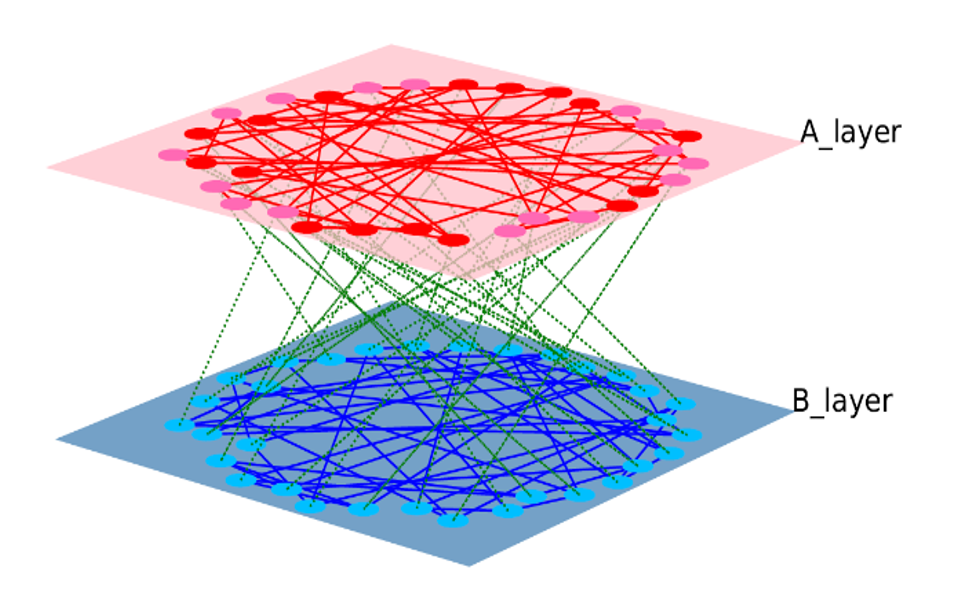
\includegraphics[width=\hsize]{FIG1.png}
  \caption{Competing Interconnected Network}
  \label{Fig1}
\end{figure}

\section{Simulation Result}
    We organized interconnection networks in Section 2. Each layer consists of a random regular network that each node has same degree.[15] Each node has five internal edges and one external edge. Layer A dynamics have the probability p and probability q denoted by M-model. We observe how the state changes by switching the probability p and probability q. To simply represent the probability p and probability q as one value, we set the value to p+q=1, and the $\gamma$ = p/q. $\gamma$ represents the strength of opinion.[9] For layer B dynamics, by switching $\beta$, we investigate the change of states. $\gamma$ scale is from 0 to 2, and $\beta$ scale is from 0 to 3, basically. But, $\beta$ scale depends on the number of degrees. So, when the number of degrees is changed, the $\beta$ scale would be adjusted properly to basic model scale.
Among the two dynamics, layer A dynamics are preceded first, and then layer B dynamics are implemented. When each dynamic is performed, one step ends. Basically, 30 steps are taken. And the same procedure is repeated 100 times to calculate the average of each layer states.
The `Average state of layer A and B' is calculated by summing the average of layer A state and the average of layer B state. With `Average state of layer A and B', we can check whether the consensus happen or not in accordance with $\gamma$ and $\beta$ changing.  If the positive consensus happens, it would be close to the value of 3, summation of layer A node average state(+2) and layer B node average state(+1) , and if the negative consensus happens, it would be close to the value of -3, summation of layer A node(-2) and layer B node(-1). The value between 3 and -3 is not on the consensus yet, so the states of positive and negative are on the coexistence part.
First, the basic model is simulated, and then other simulation would be implemented with revised network structure.

\subsection{Basic Model Result}
Basic model simulation result is like Fig2 and Fig3.
\begin{figure}[!htb]
  \centering
  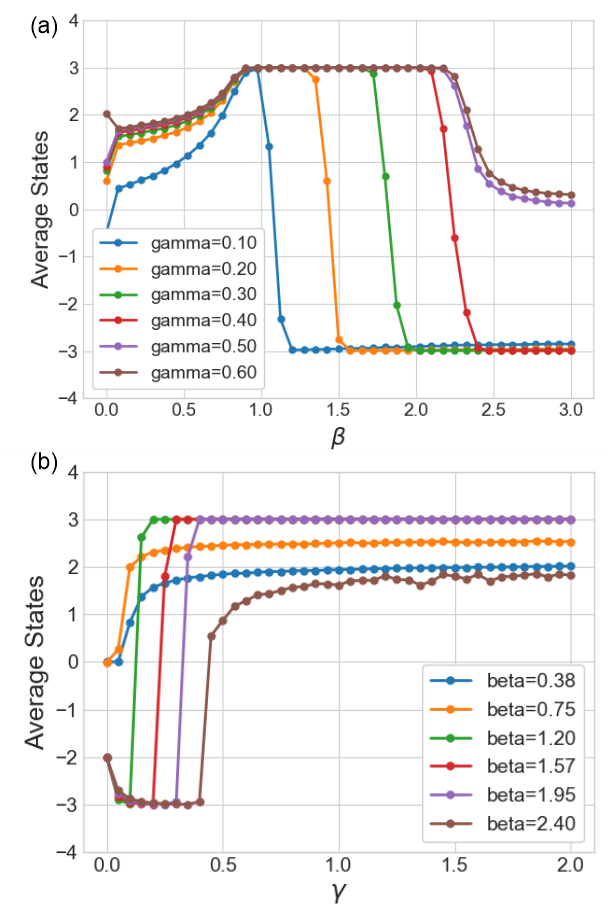
\includegraphics[width=\hsize]{FIG2.png}
  \caption{(a) $\beta$-Average state of layer A and B chart according to some $\gamma$ values. (b) $\gamma$-Average state of layer A and B chart according to some $\beta$ values.}
  \label{Fig2}
\end{figure}

In Fig.2(a), as it shows, As $\beta$ increase, it normally tend to make positive and negative consensus. But, when $\gamma$ is very low, it can’t make positive consensus, when $\gamma$ is large enough, it can make positive consensus. But, when $\beta$ is large enough, it is changed into negative consensus. When both of $\gamma$ and $\beta$ are large enough, it has coexistence for positive and negative states.

In Fig.2(b), As $\gamma$ increase, it normally tends to make positive consensus. But, when $\beta$ is very low, it can’t make consensus. And when $\beta$ is large enough, though $\gamma$ is large enough, it cannot make positive consensus and has a coexistence part.

In Fig.3, it shows the states of two layers according to $\gamma$ and $\beta$. The X-axis is the $\gamma$ and the Y-axis is the $\beta$, and the Z-axis represents the average sum of the nodes' states in layer A and B.

\begin{figure}[!htb]
  \centering
  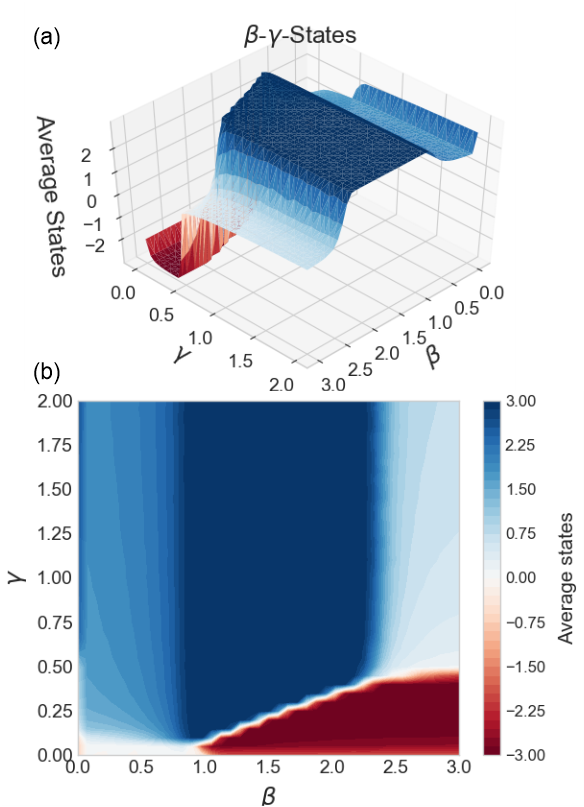
\includegraphics[width=\hsize]{FIG3.png}
  \caption{Basic model 3D result (1). (a) $\gamma$-$\beta$-Average state of layer A and B chart at angle (45, 45). (b) $\gamma$-$\beta$-Average state of layer A and B chart at angle (90, 0)}
  \label{Fig3}
\end{figure}
In Fig.3, The closer the color is blue, the closer it has positive consensus, the closer the color is red, the closer it has negative consensus. A light or white part is the parts that is not a consensus, and has coexistence part with positive and negative states. It has two light or white part, when $\beta$ is very low or very high. That means it has two transition parts such as coexistence to consensus and consensus to coexistence.

In Fig.4, the fractions of positive states are investigated on each layer. The result of layer A is like Fig.4 (a). Layer A has lots of positive parts. And the part of coexistence is very small. As the $\beta$ increases, the $\gamma$ is needed to increase for the positive consensus. As the parameter of layer A dynamics, the $\gamma$ is operating properly. The result of layer B is like Fig.4 (b). Layer B has various states as $\gamma$ and $\beta$ change. But, Almost layer B states depends on power $\beta$.  When $\beta$ is very small, layer B states are almost in the coexistence. When $\beta$ is very large, layer B state are almost negative. When $\beta$ is in the middle$(0.8 < \beta < 2.25)$, the states are the consensus parts. The states of layer B is almost like layer A states. As the parameter of layer B dynamics, the $\beta$ is also operating properly. Fig.4 (c) is the result of the summation of (a) and (b). The chart is almost like Fig.3 result. Through this charts,
There is the difference of coexistence parts. The coexistence with small $\beta$ is due to inner competition of layer B. The coexistence with large $\beta$ is due to outer competition between layer A and layer B
\begin{figure}[!htb]
  \centering
  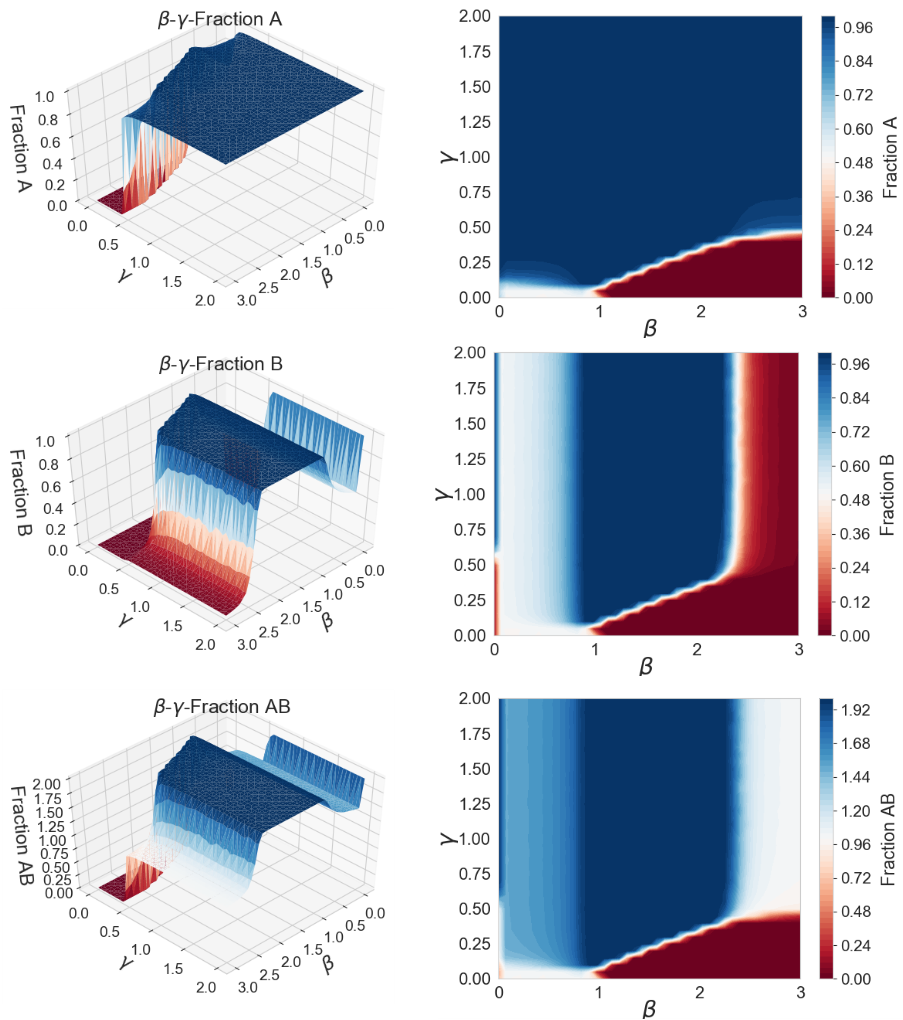
\includegraphics[width=\hsize]{FIG4.png}
  \caption{Basic model 3D result (2) (a) $\gamma$-$\beta$-Fraction A chart. ‘Fraction A’ means the fraction of positive states in the layer A. (b) $\gamma$-$\beta$-Fraction B chart. ‘Fraction B’ means the fraction of positive states in the layer B. (c) $\gamma$-$\beta$-Fraction AB chart. ‘Fraction AB’ means the summation of Fraction A and Fraction B.}
  \label{Fig4}
\end{figure}
\subsection{Leader Model Result}
 The leader model is the model to reduce the number of nodes in layer B from 2048 to 128 while increase the number of external edges by 16 times as the number of nodes in the node decreases by 1/16.  In other words, each layer A node has one external item, but each layer B node has 16 external edges. That is, one node of layer B represents the 16 nodes. $\gamma$ scale is same with the basic model. But, $\beta$ scale depends on the number of degrees. So the $\beta$ scale is adjusted to same property with the basic model.
The leader model simulation results are like this Fig.5
Comparing with Basic Model, white or light parts, that is coexistence parts, are decreased remarkably. And it has only 1 transition part where $\beta$ is large enough. It shows that leader model has more consensus parts than basic model.
\begin{figure}[!htb]
  \centering
  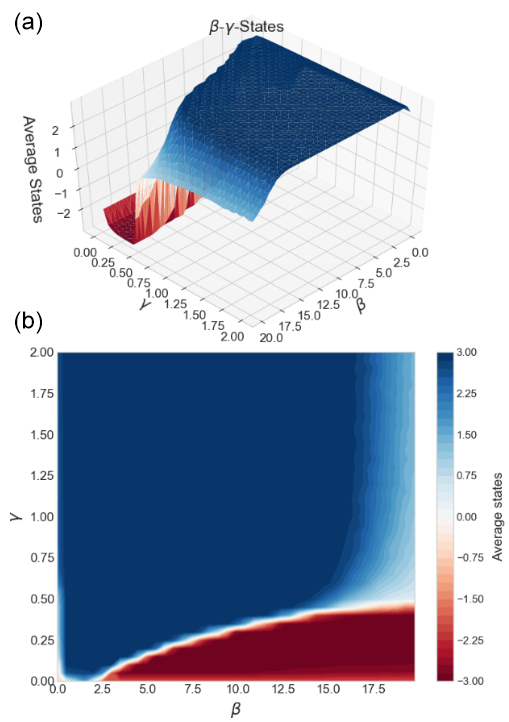
\includegraphics[width=\hsize]{FIG5.png}
  \caption{Leader Model 3D result. (a) $\gamma$-$\beta$-Average state of layer A and B chart at angle(45, 45). (b) $\gamma$-$\beta$-Average state of layer A and B chart at angle(90, 0)}
  \label{Fig5}
\end{figure}
\subsection{Different Structure Network Model}
So far, each layer of the interconnected network consist of random regular network that has the same number of edges for the nodes. Now, the simulation would be implemented with Barabasi-Albert network[16, 17]. For this simulation, each layer has 2048 nodes, 1 external edges for each each node. The internal edges depend on Barabasi-Albert network(BA). So it has total 615 edges for each layer(BA is set up as average 5 internal edges), it has more 295 edges than the random regular network(RR) that has total 320 internal edges(RR is set up as 5 internal edges for each node). The simulation would be carried out, with switching each layer to RR or BA network structure.
In Fig. 6 (a) and (b), (b) result has more white part(coexistence) than (a) result. That means increasing internal edges in both layers makes more coexistence part.
In Fig. 6 (c), comparing with (a), the red part(negative consensus) is decreased and the blue part(positive consensus) is increased. Since Layer A is BA that has more internal edges, it seems to be more power to keep layer A states.
In Fig. 6 (d), comparing with (a), the red part and white part are increased. Since Layer B is BA that has more internal edges, it seems to be more power to keep layer B states.
\begin{figure}[!htb]
  \centering
  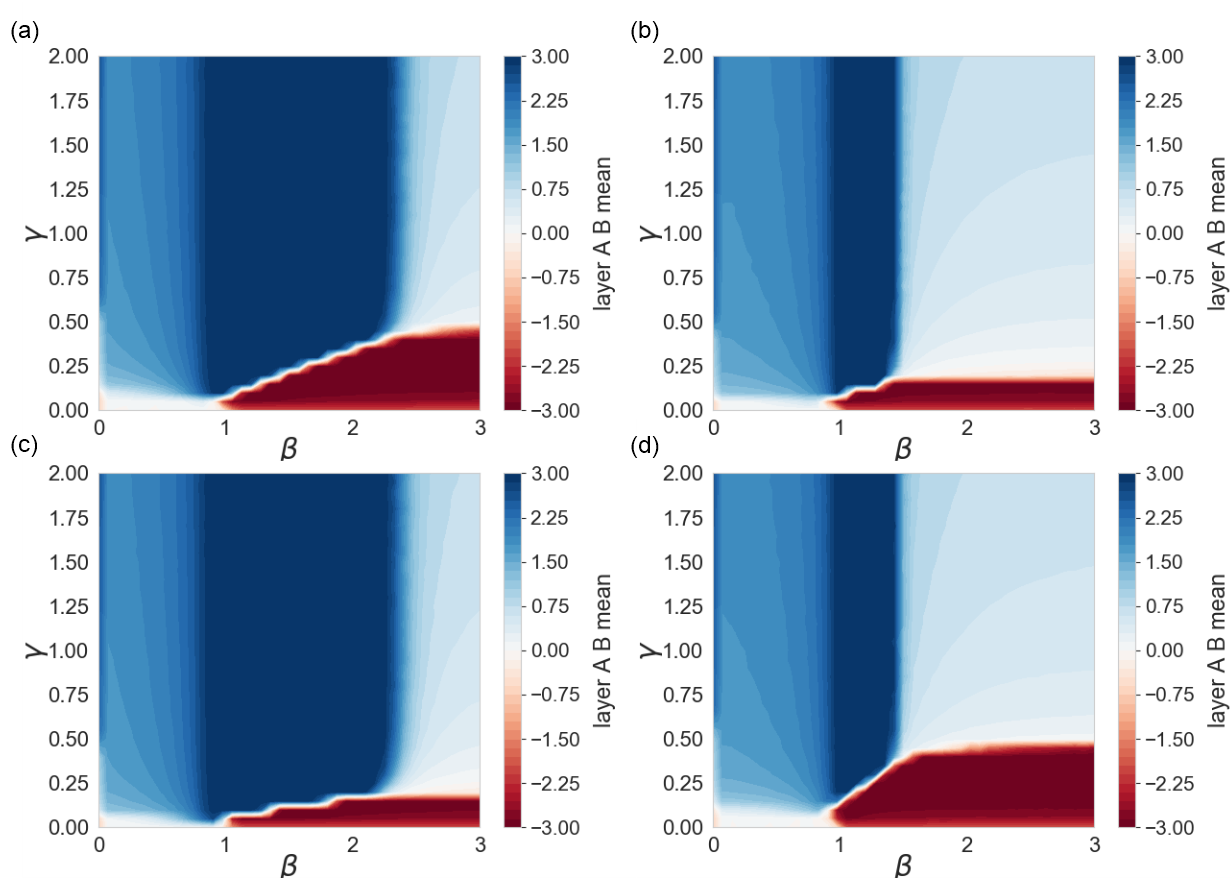
\includegraphics[width=\hsize]{FIG6.png}
  \caption{The simulation results for interconnected network with different structure network (a) layer A(RR)-layer B(RR), (b) layer A(BA)-layer B(BA), (c) layer A(BA)-layer B(RR), (d) layer A(RR)-layer B(BA)}
  \label{Fig6}
\end{figure}

In order to confirm that the number of internal edges affects consensus, The internal edges of layer A and B change to 2 or 5. The simulation is carried out with only RR networks that has total 320 or 128 internal edges on layer. The result is like this Fig 7.
\begin{figure}[!htb]
  \centering
  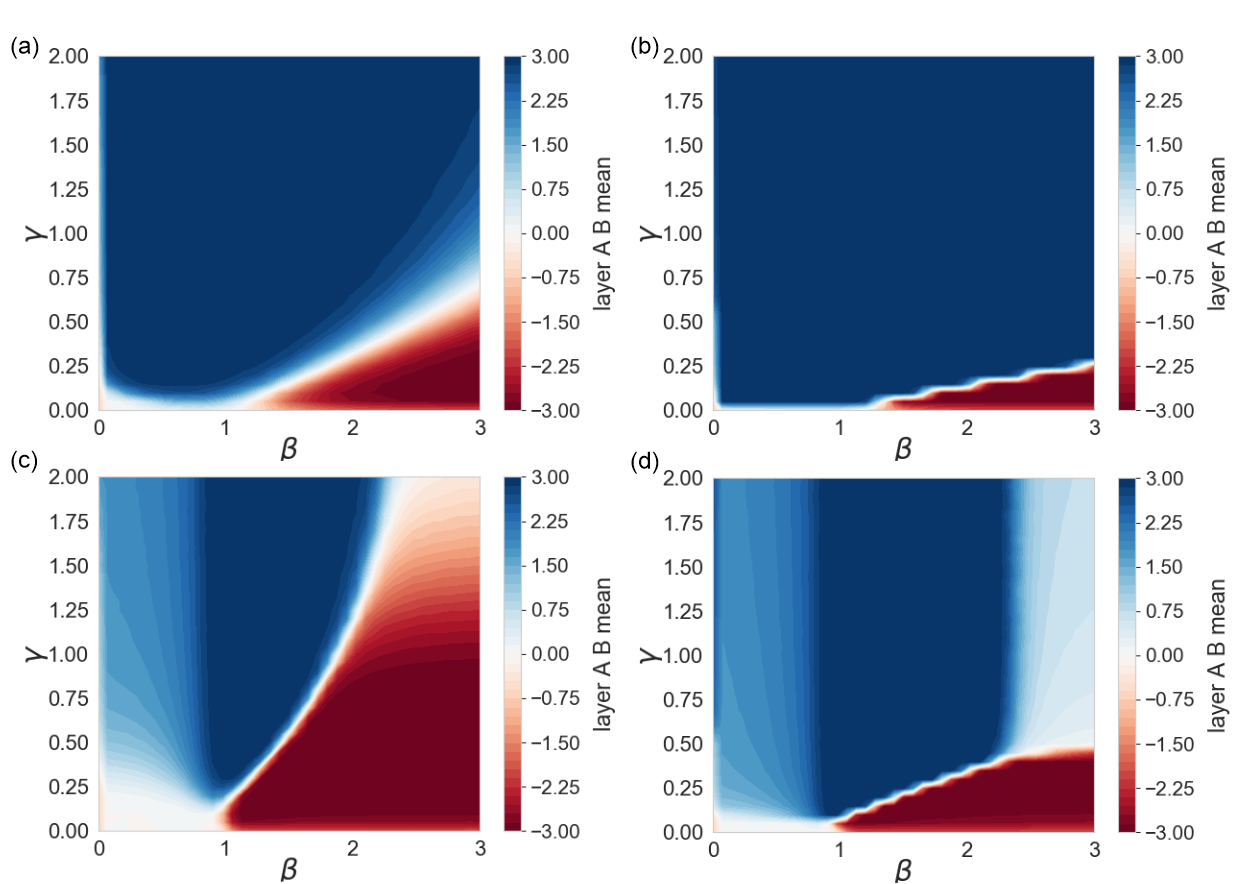
\includegraphics[width=\hsize]{FIG7.png}
  \caption{Consensus Comparison according to changing the number of internal edges on layer A and B (a) RR(128)-RR(128), (b) RR(320)-RR(128), (c) RR(128)-RR(320), (d) RR(320)-RR(320)}
  \label{Fig7}
\end{figure}
As we can see the result, we can find out the number of internal edges affects consensus. In Fig.7 (b) RR(320)-RR(128), it has decreased red part(negative consensus) and increased blue part(positive consensus). That means that layer A has more power than layer B. As the internal edges on layer A increase, the red part get smaller and the blue part get larger.
Inversely, in Fig. 7 (c) RR(128)-RR(320), it has increased red part(negative consensus) and decreased blue part(positive consensus). That means that layer B has more power than layer A.
Next, in order to compare BA network with RR network that has the similar number of edges, The internal edges of RR network are increased to the similar number of BA network internal edges. The simulation was carried out with RR network that has total 640 internal edges on layer A(layer B has RR network with 320 internal edges). The result is like Fig.8.
\begin{figure}[!htb]
  \centering
  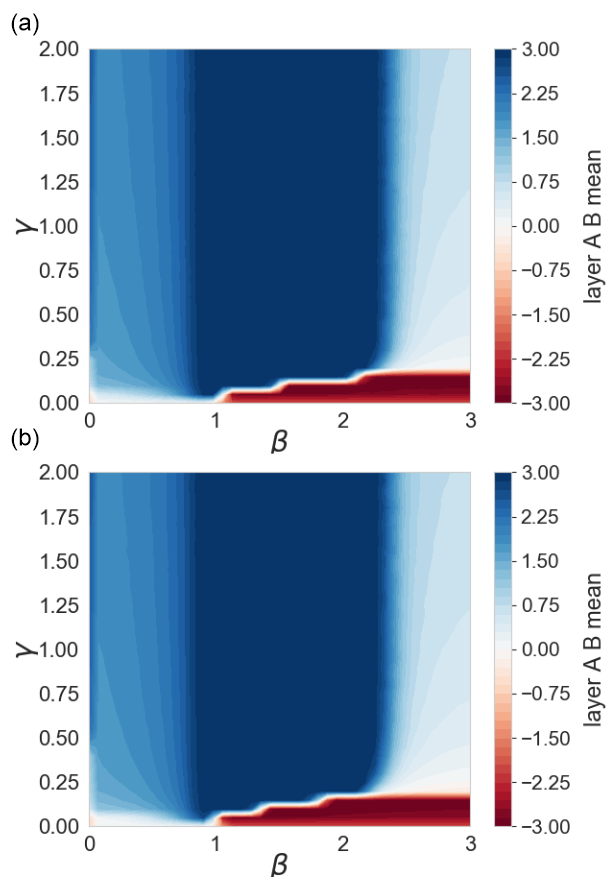
\includegraphics[width=\hsize]{FIG8.png}
  \caption{Comparison between BA network and RR network (a) RR(640)-RR(320), (b) BA(615)-RR(320)}
  \label{Fig8}
\end{figure}
In Fig. 8 (a), as you can see, BA network simulation result is almost same with RR network. We can analyze the number of edges have influence on the consensus. In other words, The network with much more edges leads to make consensus.

\subsection{Increasing The Step of Dynamics}
The basic model was implemented by 30 steps of interconnected dynamics that include opinion dynamics and decision-making dynamics. In this simulation, the number of step is increased from 30 to 100 steps. Increasing the number of steps in interconnected dynamics means the networks keeps interconnected dynamics for enough time.  In the real world, it is the same effect as increasing time.
The results of increasing the number of steps to 100 are as follows.
\begin{figure}[!htb]
  \centering
  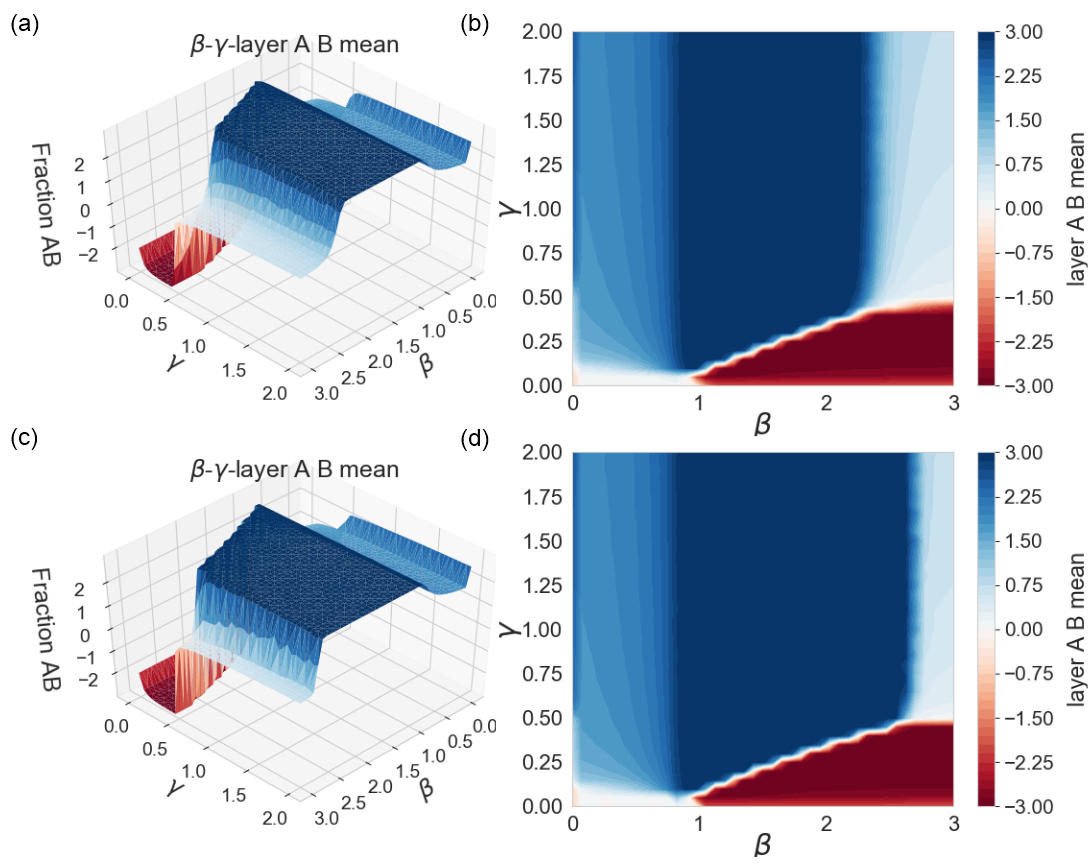
\includegraphics[width=\hsize]{FIG9.png}
  \caption{The comparison between Basic Model(30times dynamics) and Dynamics steps increased Model(100 times)}
  \label{Fig9}
\end{figure}

In Fig. 9, Dynamics steps increased Model has more blue part(positive consensus), and white part(coexistence) is decreased. That means consistent social opinion can make consensus with its state.

\begin{figure*}[!htb]
  \centering
  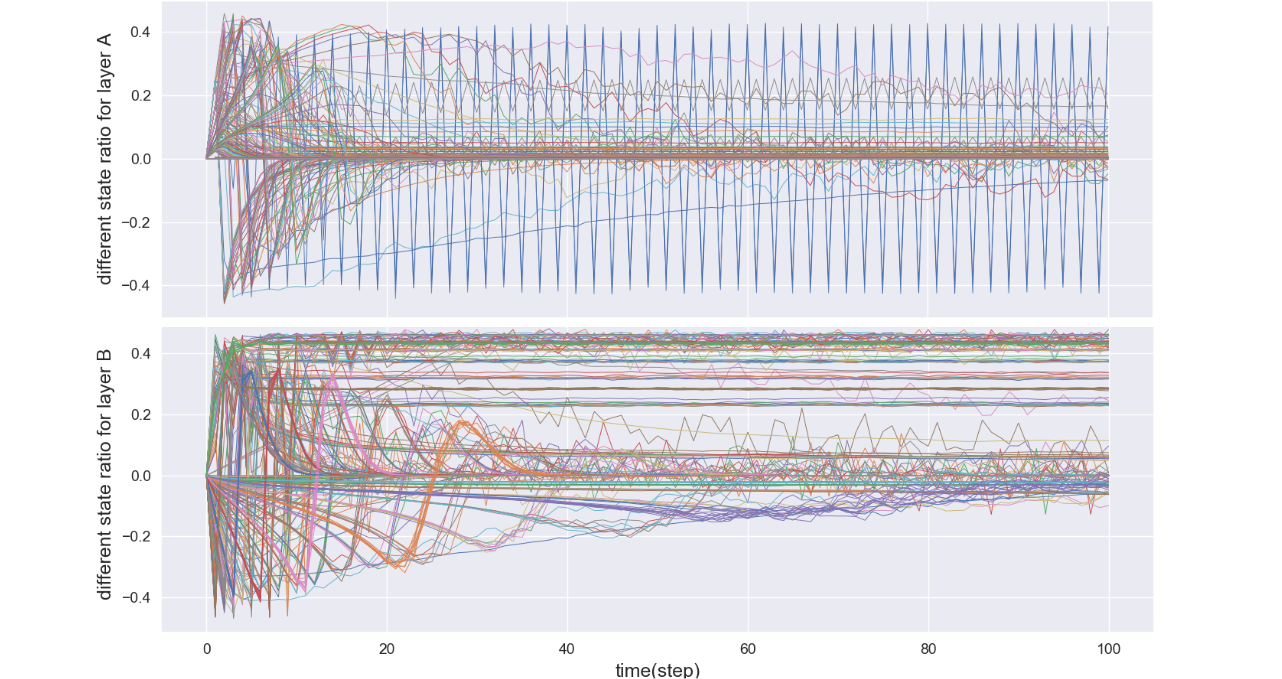
\includegraphics[width=\hsize]{FIG10.png}
  \caption{Time evolution of the fraction of nodes in different states on layer A and layer B, the ratio of different state means the fraction of the number of different state node for each layer. The sign of ratio depends on the major nodes on each layer. For example, if the major nodes on layer A are negative, the sign of that ratio is negative.}
  \label{Fig10}
\end{figure*}
In Fig. 10, the charts show that most of ratios on the layer A are approaching to 0 with steps proceeding, except the case that volatility is very large. The ratios on the layer B are divided by some values. But except some values, they are approaching to 0. That means two layers can make consensus by proceeding the steps with stable $\gamma$ and $\beta$.

\section{Comparison and Analysis}
In this section, the simulation results are compared and analyzed, and then it would be found out what conditions make the consensus on the interconnected networks.
If the leader model compares with the basic model, we can see that the leader model has more consensus part than the basic model (white part is less than basic model). And the basic model has two transition parts, but the leader model has just one transition part. This means that the base model has transition parts when the $\beta$ is very small or very large. But in case of the leader model, though $\beta$ is very small, the consensus is easy to make. Only if $\beta$ is very large, the consensus is hard to happen.
The next comparison is models with different structure networks. The total number of internal edges in BA is 615, and the internal edges in RR are total 320. This comparison simulation shows how the number of internal edges affects interconnected dynamics. First, when we check the BA-RR and RR-BA simulation results, we can see that it makes the more consensus with BA network layer states than RR-RR simulation.  In other words, the layer with more internal edges seems to have more power to maintain its own state. That is, interconnected networks tend to make consensus with the layer that has more internal edges. RR-RR simulation results have more consensus parts than BA-BA simulation results. we can analyze that BA-BA simulations result in poor consensus due to having a strong power to maintain their both states. And, BA network was compared with RR network that has the similar number of internal edges. The result is almost same. It can be analyzed that the network with more edges have more power to keep their states and make consensus for its states.
The next analysis is a comparison with a model that increases the number of steps in the dynamic. A model that increases the number of steps can be seem to have more consensus with layer A. In other words, it means that social opinion is likely to achieve the consensus if it is given enough time. (Of course, if the volatility is too low or too high, it would not make consensus.)
Through these three comparisons and analysis, we can provide three conditions that increase the likelihood of consensus with social opinion. First, as we can see the case of leader model, if reducing the node in the decision-making layer and increasing the external edges, we can increase the probability of consensus. Second, as different network structure comparisons show, for positive consensus, it is needed to have more internal edges than opposite layer. Because increasing the internal edges of social opinion is likely to have more power to keep the states. Third, as shown by the model that increased the number of dynamic steps, if given enough time, there is a high possibility of consensus with social opinion.

\section{Conclusion}
In this work, we have researched competing interconnected network dynamics. Layer A is a layer of social opinion and has positive states as an initial condition. It is influenced by opinion dynamics. Layer B is a network representing decision making system and has a negative state as an initial condition. It is influenced by the language competition dynamics. When these two layers were connected and interacted, it was researched and analyzed how their states were changed with switching $\gamma$ and $\beta$.
In the basic model, the simulation result shows the negative consensus, the positive consensus, and the coexistence sections according to $\gamma$ and $\beta$
Based on these basic models, we presented and simulated leader model, different structure networks model, and model with increased number of dynamic steps. As a result, we found out three conditions that increase the likelihood of consensus with social opinion layer. The first is to reduce nodes in the decision-making layer and increase the external edges like the leader model. The second is to increase the internal edges of social opinion in order to strengthen the power to maintain its state. But too many internal nodes can make internal conflicts. The third is to take enough time and keep social opinion with enough $\gamma$.
More research will be needed to make generalized model and to be applied to real social networks. we think this research can contribute to providing the characteristics of the system and the framework of social networks analysis such as the legalization or social decision-making system, and we hope it help the research on interconnected networks and multi-layer networks. As the forward work, it would be very interesting to make the generalized model for competition of interconnected network.

\begin{thebibliography}{0}
\bibitem{newman2010}
M. E. J. Newman, Networks: An Introduction, Oxford University Press, 2010.


\bibitem{boccaletti2014}
S. Boccaletti et al. The structure and dynamics of multilayer networks, Physics Reports 544, pp.1, 2014.

\bibitem{domenico2013}
M. De Domenico et al. Mathematical Formulation of Multilayer Networks, Physical Review X 3, pp.1, 041022, 2013.


\bibitem{tomasini2015}
Marcello Tomasini . An Introduction to Multilayer Networks. 10.13140/RG.2.2.16830.18243, 2015.

\bibitem{namkhanhvu2017}
Nam Khanh Vu, Robustness of Interconnected Complex Networks with Directed Dependency, June 2017.

\bibitem{mikko2013}
Mikko Kivela et al. Multilayer Networks. SSRN Electronic Journal. 2. DOI : 10.1093/comnet/cnu016, 2013.


\bibitem{halu2013}
A. Halu, K. Zhao et al. Dynamic interdependence and competition in multilayer networks, EPL(Europhysics Letters) 102, 16002, URL http://stacks.iop.org/0295-5075/102/i=1/a=16002, pp.1-5, 2013.


\bibitem{bianconi2018}
G. Bianconi, Multilayer Networks: Structure and Function, Oxford University Press, 2018.

\bibitem{alvarez2016}
Alvarez-Zuzek et al. Interacting Social Processes on Interconnected Networks. PLoS ONE. 11. 10.1371/journal.pone.0163593, 2016.


\bibitem{gomez2015}
Gomez Gardenes J. et al. Layer-layer competition in multiplex complex networks. Phil. Trans. R. Soc. A 373:20150117, 2015

\bibitem{diep2017}
H.T. Diep et al. Dynamics of two-group conflicts: A statistical physics model, Physica A, http://dx.doi.org/10.1016/j.physa.2016.10.072, 2017.


\bibitem{rocca2014}
C. E. La Rocca et al. The influence of persuasion in opinion formation and polarization, Europhys. Lett. 106, 40004, pp.1-2, 2014.


\bibitem{abrams2003}
M Abrams et al. Modelling the dynamics of language death. Nature.424.900. DOI : 10.1038/424900a, 2003.


\bibitem{vazquez2010}
 F. Vazquez et al. Agent based models of language competition: macroscopic descriptions and order–disorder transitions, Journal of Statistical Mechanics: Theory and Experiment 2010, P04007, 2010.


\bibitem{bela2001}
 Bela Bollobas, Random Graphs, 2nd edition, Cambridge University Press, section 2.4: Random Regular Graphs, 2001.


\bibitem{barabasi1999}
Barabasi, A. L., and Albert, R., Emergence of Scaling in Random Networks, Science 286, 509, DOI: 10.1126/science.286.5439.509, 1999.
Kim Sangwoo, Structure and dynamics of complex networks, Yonsei Univ, 2012.

\bibitem{kimsangwoo2012}
Kim Sangwoo, Structure and dynamics of complex networks, Yonsei Univ, 2012.


\end{thebibliography}

\end{document}



































